% !TEX root = ../Thesis.tex
\chapter{Top-quark physics} \label{sec:top_quark_physics}
The third generation of quarks was first proposed by Kobayashi and Maskawa in a paper published in 1973~\cite{Theory:CKMKobayashiMaskawa} as a way to exaplain the $CP$ violation observed in Kaon decays. The existence of the third generation was confirmed when the lighter of the two constituents, the $b$ quark, was discovered in 1977~\cite{Top:bQuarkDiscovered}.

Due to its large mass, direct confirmation of the existence of the top quark required the construction of very powerful accelerators. The top quark was discovered by the CDF and D0 experiments at Fermilab in 1995~\cite{Top:ObservationCDF,Top:ObservationD0}.

Its large mass makes the top quark a very interesting object of study. The current world average for the mass of the top is $m_{t}=173.07\pm0.52\pm0.72$ GeV based on results from Tevatron and the LHC~\cite{Theory:PDGBooklet}. Due to its mass the top quark has an extremely short lifetime $\tau\approx0.5\times10^{-24}$ s, too short to interact via the strong force and hadronize into a bound state~\cite{Theory:TopQuarkDecayTooQuickly}. Instead the top quark decays weakly producing a $W$ boson and a $b$ quark almost exclusively. This allows experimentalist to directly study the properties of a bare quark. An impossibility with the other quarks which bind with other quarks to form hadrons. Measurement of top quark properties (mass, charge, forward-backward asymmetry, couplings, etc...) forms a large part of high energy physics research. Measurement of these properties provide rigorous tests of the SM, point towards the existence of new physics or exclude some BSM theories.

From an experimental perspective, top quark decays can produce a very interesting signature which includes leptons, jets and missing energy due to the escaping neutrino\footnote{Neutrinos do not interact with the detector material and thus escape without being detected}. The study of top quark decays relies on all parts of a general purpose detector such as ATLAS or CMS. In additional \ttbar\ pair production constitutes a background for many other SM and BSM searches, as such understanding this process well is fundamental for almost all areas of HEP research.

\section{Top quark production} \label{sec:top_quark_production}

Top quarks can be produced in two manners, single top production and \ttbar\ pair production. In hadron colliders production dominantly takes place via the strong force through $qq \rightarrow t\bar{t}$ and $gg \rightarrow t\bar{t}$ at leading order. The feynman diagrams for these interactions are shown in Figure~\ref{fig:TopQuarkProduction}. \comment{MENTION THEORETICAL MEASUREMENTS OF XSECTION AND TEVATRON VS LHC}

% tt-bar pair production plots
\begin{figure}[tbph]
  \centering
  \begin{minipage}[][][t]{.47\textwidth}
    \centering
    % !TEX root = ../../Thesis.tex
\begin{fmffile}{TopProdStraightgg2tt}
\fmfframe(5,17)(20,17) {
\begin{fmfgraph*}(150,70)
\fmfleft{gluon1,gluon2}
\fmfright{tbar,top}
\fmf{gluon}{gluon1,v1}
\fmf{gluon}{gluon2,v2}
\fmf{fermion}{tbar,v1}
\fmf{fermion,tension=0}{v1,v2}
\fmf{fermion}{v2,top}
\fmflabel{$g$}{gluon1} \fmflabel{$t$}{top}
\fmflabel{$g$}{gluon2} \fmflabel{$\overline{t}$}{tbar}
\end{fmfgraph*}
}
\end{fmffile}
    \subcaption{Gluon fusion (t-channel)}
  \end{minipage}
  \,
  \begin{minipage}[][][t]{.47\textwidth}
    \centering
    % !TEX root = ../../Thesis.tex
\begin{fmffile}{TopProdCrossGG2ttbar}
\fmfframe(5,17)(20,17) {
\begin{fmfgraph*}(150,70)
\fmfleft{i1,i2}
\fmfright{o1,o2}
\fmf{gluon}{v1,i1}
\fmf{phantom}{v1,o1} % Invisible rubber band
\fmf{gluon}{v2,i2}
\fmf{phantom}{v2,o2} % also invisible rubber band
\fmf{fermion,tension=0}{v1,v2}
% These are visible, but have no tension.
\fmf{fermion,tension=0}{o2,v1}
\fmf{fermion,tension=0}{v2,o1}
\fmflabel{$g$}{i1}
\fmflabel{$g$}{i2}
\fmflabel{$t$}{o1}
\fmflabel{$\overline{t}$}{o2}
\end{fmfgraph*}
}
\end{fmffile}
    \subcaption{Gluon fusion (u-channel)}
  \end{minipage}
  
  \begin{minipage}[][][t]{.47\textwidth}
    \centering
    % !TEX root = ../../Thesis.tex
\begin{fmffile}{TopProdgg2g2ttbar}
\fmfframe(5,17)(5,17) {
\begin{fmfgraph*}(150,70)
\fmfleft{gluon1,gluon2}
\fmfright{top1,top2}
\fmf{gluon}{v1,gluon1}
\fmf{gluon}{v1,gluon2}
\fmf{gluon,label=$g$,l.d=10}{v2,v1}
\fmf{fermion}{top1,v2,top2}
\fmflabel{$g$}{gluon1} \fmflabel{$t$}{top2}
\fmflabel{$g$}{gluon2} \fmflabel{$\bar{t}$}{top1}
\end{fmfgraph*}
}
\end{fmffile}
    \subcaption{Gluon fusion (s-channel)}
  \end{minipage}
  \,
  \begin{minipage}[][][t]{.47\textwidth}
    \centering
    % !TEX root = ../../Thesis.tex
\begin{fmffile}{TopProdqq2ttbar}
\fmfframe(5,17)(5,17) {
\begin{fmfgraph*}(150,70)
\fmfleft{q,qbar}
\fmfright{tbar,top}
\fmf{fermion}{qbar,v1,q}
\fmf{gluon,label=$g$,l.d=10}{v2,v1}
\fmf{fermion}{tbar,v2,top}
\fmflabel{$q$}{q} \fmflabel{$t$}{top}
\fmflabel{$\bar{q}$}{qbar} \fmflabel{$\bar{t}$}{tbar}
\end{fmfgraph*}
}
\end{fmffile}
    \subcaption{Quark pair annihilation}
  \end{minipage}
  \,
  \caption{The leading order Feynman diagrams for \ttbar\ production.}
  \label{fig:TopQuarkProduction}
\end{figure}

Single top production occurs via the weak force almost exclusively through the $Wtb$ vertex. The leading order weak interactions are shown in Figure~\ref{fig:TopSingleProduction}. As top quark pair production can proceed via the strong force it occurs overwhelmingly more often than single top production. 

% single top production plots
\begin{figure}[tbph]
  \centering
  \begin{minipage}[][][t]{.47\textwidth}
    \centering
    % !TEX root = ../../Thesis.tex
\begin{fmffile}{TopSingleTopSChannel}
\fmfframe(5,17)(20,17) {
\begin{fmfgraph*}(150,70)
\fmfleft{quark,antiquark}
\fmfright{top,bbar}
\fmf{fermion}{quark,v1,antiquark}
\fmf{boson,label=$W$}{v1,v2}
\fmf{fermion}{bbar,v2,top}
\fmflabel{$q$}{quark} \fmflabel{$t$}{top}
\fmflabel{$\overline{q'}$}{antiquark} \fmflabel{$\overline{b}$}{bbar}
\fmfdot{v1,v2}
\end{fmfgraph*}
}
\end{fmffile}
    \subcaption{s-channel} \label{fig:TopSingleSChannel}
  \end{minipage}
  \,
  \begin{minipage}[][][t]{.47\textwidth}
    \centering
    % !TEX root = ../../Thesis.tex
\begin{fmffile}{TopSingleTWChannel}
\fmfframe(5,17)(20,17) {
\begin{fmfgraph*}(150,70)
\fmfleft{gluon,b}
\fmfright{top,W}
\fmf{gluon}{gluon,v1}
\fmf{fermion}{b,v1}
\fmf{fermion,label=$b$}{v1,v2}
\fmf{fermion}{v2,top}
\fmf{boson}{v2,W}
\fmflabel{$g$}{gluon} \fmflabel{$t$}{top}
\fmflabel{$b$}{b} \fmflabel{$W$}{W}
\end{fmfgraph*}
}
\end{fmffile}
    \subcaption{$tW$-channel} \label{fig:TopSingletWChannel}
  \end{minipage}

  \begin{minipage}[][][t]{.47\textwidth}
    \centering
    % !TEX root = ../../Thesis.tex
\begin{fmffile}{TopSingleQtb}
\fmfframe(5,17)(18,17) {
\begin{fmfgraph*}(150,70)
\fmfleft{glu1,quark}
\fmfright{bbar,top,qprime}
\fmf{fermion}{quark,v1,qprime}
\fmf{gluon}{v3,glu1}
\fmf{fermion}{bbar,v3}
\fmffreeze
\fmf{phantom}{v1,v3}
\fmf{boson,label=$W$}{v1,v2}
\fmf{fermion,label=$b$}{v3,v2}
\fmffreeze
\fmf{fermion}{v2,top}
\fmflabel{$g$}{glu1} \fmflabel{$t$}{top}
\fmflabel{$q$}{quark} \fmflabel{$q'$}{qprime} \fmflabel{$\bar{b}$}{bbar}
\end{fmfgraph*}
}
\end{fmffile}
    \subcaption{Associated with a $q$ and $\bar{b}$} \label{fig:TopSingleqtbChannel}
  \end{minipage}
  \,
  \begin{minipage}[][][t]{.47\textwidth}
    \centering
    % !TEX root = ../../Thesis.tex
\begin{fmffile}{TopSingleqb2qt}
\fmfframe(5,17)(5,17) {
\begin{fmfgraph*}(150,70)
\fmfleft{ib,iq}
\fmfright{ot,oq}
\fmf{fermion}{iq,v1,oq}
\fmf{fermion}{ib,v2,ot}
\fmffreeze
\fmf{boson,label=$W$}{v1,v2}
\fmflabel{$b$}{ib} \fmflabel{$t$}{ot}
\fmflabel{$q$}{iq} \fmflabel{$q'$}{oq}
\end{fmfgraph*}
}
\end{fmffile}
    \subcaption{Associated with a $q$} \label{fig:TopSingleqtChannel}
  \end{minipage}
  \caption{Example Feynman diagrams for single top quark at leading order.}
  \label{fig:TopSingleProduction}
\end{figure}

\section{Top quark decay modes} \label{sec:top_quark_decay_modes}

The top quark decays almost exclusively into a $W$ boson and a $b$-quark. The ratio of branching ratios $\Gamma(t\rightarrow Wb)/\Gamma(t\rightarrow Wq(q=b,s,d))$ is $0.91\pm0.04$~\cite{Theory:PDGBooklet}.

As the LHC collides proton-proton beams, the overwhelming majority of events produced will feature multiple hadronic \textit{jets}, a stream of particles resulting from the hadronization of quarks in the detector, most of which will originate from ``light'' quarks\footnote{The term light quarks usually refers to quarks in the first two generations. Light jets are those originating from those quarks}. Unlike these light quarks, $b$ quarks leave a distinct signature in the detector as they travel a certain distance within a $B$ hadron before producing a jet. Additional features such as the semi-leptonic decay of $b$ quarks can be exploited to determine the presence of such a quark in the detector. Collectively analysis techniques that permit the detection of $b$-jets are known as \textit{b-tagging}. Top quark events will produce two $b$ quarks, making b-tagging techniques a central part of any \ttbar\ analysis.

The other part of the top decay, the $W$ boson is used to classify \ttbar\ events. As discussed in Section~\ref{sec:the_standard_model_of_particle_physics}, $W$ bosons can decay leptonically ($\ell\nu_{\ell}$) or hadronically ($W\rightarrow q\bar{q}'$) driven by the CKM vertex element, since $\Gamma\propto|V_{ij}|^2$. The various branching ratios of $W$ decays are presented in Table~\ref{tab:TopQuakWDecayBranchingRatios}.

\begin{table}
  \centering
  \begin{tabular}{|c|c|}
    \hline
    Decay      & Branching ratio \\ \hline\hline
    $W\rightarrow e+\nu$    & $(10.75\pm0.13)\%$ \\
    $W\rightarrow \mu+\nu$  & $(10.57\pm0.15)\%$ \\
    $W\rightarrow \tau+\nu$ & $(11.25\pm0.20)\%$ \\
    hadrons    & $(67.60\pm0.27)\%$ \\
    \hline
  \end{tabular}
  \caption{Branching ratios for the decay of $W$ boson. Note that the ``hadrons'' refers to a possible combination of $q\bar{q}'$ where $\bar{q}'$ denotes the antiquark of a flavour different to that of the first quark.}
  \label{tab:TopQuakWDecayBranchingRatios}
\end{table}

Thus \ttbar\ events are labelled as ``dilepton'', ``all-hadronic'' or ``lepton + jets'' depending on the combination of $W$ decays present. The probability for \ttbar\ event to be of a given type is dependent on the branching-ratios of $W$ decays shown a priori. As can be seen from Figure~\ref{fig:TopQuarkDecayModes} the all-hadronic events dominate, followed by the lepton plus jets and dilepton. Each of these types requires a very different analysis approach due to their distinct backgrounds, branching-ratio, detector signature and reconstruction requirements.

\begin{figure}[tbhp]
  \centering
  \includegraphics[width=0.90\textwidth]{PartTopQuark/Diagrams/TopQuarkDecayPie.pdf}
  \caption{Branching ratios of all possible \ttbar\ decays. These probabilities are based on the branching-ratios of $W$ decay shown in Table~\ref{tab:TopQuakWDecayBranchingRatios}.}
  \label{fig:TopQuarkDecayModes}
\end{figure}

The all-hadronic final state includes four light quarks which will hadronize to form four Light Flavour (LF) jets and two $b$ quarks leading to two $b$ jets. Due to the large hadronic activity the all-hadronic channel is very challenging. As mentioned before, hadronic collisions produce events with a large number of quarks -- and thus jets -- in the final state. The background to the all-hadronic channel are therefore very high. As shown in Figure~\ref{fig:TopQuarkDecayModes}, the all-hadronic channel has the largest branching ratio of the three.

The dilepton final state includes two leptons, large missing energy from two neutrinos which escape the detector and two $b$ jets. In constrast to the all-hadronic channel, dilepton events are very clean due to the presence of leptons and missing energy, however the branching ratio is very small and reconstruction of the top is challenging do the presence of two neutrinos which escape the detector without interacting.

Finally, the lepton plus jets channel has a large branching ratio while having a distinct signature with an isolated lepton\footnote{A lepton produced far from other physics objects (jets, leptons, etc...)} and missing energy as well as LF and $b$ jets. Typical lepton plus jets are shown in  Note that leptons in this case refers to $e$ and $\mu$ and excludes the $\tau$. The $\tau$ lepton is unstable and sufficiently heavy to decay haronically via the weak force producing two quarks, losing the advantageous distinct signature of a lepton plus jets event. An example of the full lepton plus jets chain is shown in Figure~\ref{fig:TopQuarkFullLPlusJets}.

\begin{figure}[thbp]
  \centering
  \begin{subfigure}[t]{0.30\textheight}
    \includegraphics[height=0.30\textheight]{PartTopQuark/Diagrams/atlas-2010-063-fig_09.png}
    \caption{\ttbar$\rightarrow$dilepton event at ATLAS } \label{fig:TopQuarkEventDisplayAtlas}
  \end{subfigure} %
  \hfill
  \begin{subfigure}[t]{0.30\textheight}
    \includegraphics[height=0.30\textheight]{PartTopQuark/Diagrams/cms-mu4Jets_140124_1749068_RPhi.png}
    \caption{\ttbar$\rightarrow\ell$+jets event at CMS} \label{fig:TopQuarkEventDisplayCMS}
  \end{subfigure}%
  \caption{Example event displays of \subref{fig:TopQuarkEventDisplayAtlas} a dilepton \ttbar\ event recorded by ATLAS and \subref{fig:TopQuarkEventDisplayCMS} a $\ell$+jets event recorded at CMS.} \label{fig:TopQuarkEventDisplay}
\end{figure}

\subsection{Motivations for selecting the $\ell$+jets channel}

Due to its distinct signature and high branching ratio the lepton plus jets channel was chosen as the focus for the analyses presented in this thesis. Additionally the presence of only one neutrino allows for a reconstruction of the mass of the leptonic top (the top whose associated $W$ decays leptonically) in the transverse plane and a full mass reconstruction of the top mass on the hadronic side\footnote{The methods used for this mass reconstruction is complex and not discussed in this thesis}.

\begin{figure}[htbp]
  \centering
  \begin{minipage}[][][t]{.60\textwidth}
  % !TEX root = ../../Thesis.tex
\begin{fmffile}{TopQuarkLeptonPlusJetsFull}
\fmfframe(5,17)(20,17) {
\begin{fmfgraph*}(200,200)
\fmfstraight
\fmfleft{dummy1,gluon1,gluon2,dummy2}
\fmfright{q,antiq,b,antib,lep,nu}
\fmf{gluon}{v1,gluon1}
\fmf{gluon}{v1,gluon2}
\fmf{gluon,label=$g$,l.d=10}{v2,v1}
\fmf{fermion,label=$t$,l.d=-14,tension=0.5}{top,v2}
\fmf{fermion,label=$\bar{t}$,tension=0.5}{v2,antitop}
\fmf{fermion,tension=0,tension=0}{antib,antitop}
\fmf{boson,label=$W$,tension=0}{antitop,leptonicW}
\fmf{fermion}{nu,leptonicW,lep}
\fmf{fermion,tension=0}{b,top}
\fmf{boson,label=$W$,tension=0}{hadronicW,top}
\fmf{fermion,tension=0}{antiq,hadronicW,q}
\fmflabel{$g$}{gluon1}
\fmflabel{$g$}{gluon2}
\fmflabel{$\bar{b}$}{antib}
\fmflabel{$b$}{b}
\fmflabel{$\bar{q}'$}{q}
\fmflabel{$q$}{antiq}
\fmflabel{$\ell$}{lep}
\fmflabel{$\nu_{\ell}$}{nu}
\end{fmfgraph*}
}
\end{fmffile}
  \end{minipage}
  \caption{The feynman diagram of lepton plus jets channel including \ttbar\ production via gluon fusion and decay with a leptonically decaying $W^+$. Note that all other production mechanisms are also considered and the final state where the $W^-$ is decayed leptonically is also taken into account.} \label{fig:TopQuarkFullLPlusJets}
\end{figure}

\section{Latest developments in top physics}

\textit{This section discusses a few of the latest measurements in the area of top quark pair production with a focus on LHC results.}

As discussed top quark decays provide the only probe to study the properties of a bare quark. Measurements of its properties provide a stringent test of the SM and could show hints of new physics from BSM theories. Moreover due to its final state signature, top quark pair production particularly in the lepton + jets channel, form the background to many searches for new physics. Additionally all parts of the detector are utilized in the reconstruction of $\ell$+jets events and as such it is possible to use these events to tune or \textit{calibrate} many analysis and reconstruction techniques.

\subsubsection{Cross-section measurement}

Measurement of the cross-section of the top quark is a benchmark test of the SM. Any statistically significant deviation from the predicted value could point to the presence of new physics. Some BSM theories posit the existence of particles which could decay to produce a \ttbar\ pair. If such theory is correct this would be observed in an increase in the cross section measured away from the predicted SM value.

Experimentally measurement of the cross-section is vital when attempting to reduce and estimate the amount of top quark background present in other analyses. Searches for the Higgs boson, exploit many different channels, many of which include \ttbar\ events as a background. The type of events predicted by the BSM theory, Supersymmetry (SUSY) include a large amount of missing energy, leptons and jets in the final state. Top quark pair events mimmick these processes and constitute a large background.

A summary of all \ttbar\ cross section measurements from the LHC is shown in Figure~\ref{fig:TopQuarkPairProductionSummaryLHC} and a comparison against the Tevatron measurement at $\sqrt{s}=1.96$ TeV is shown in Figure~\ref{fig:TopQuarkPairProductionComparison}.

\begin{figure}[htbp]
  \centering
  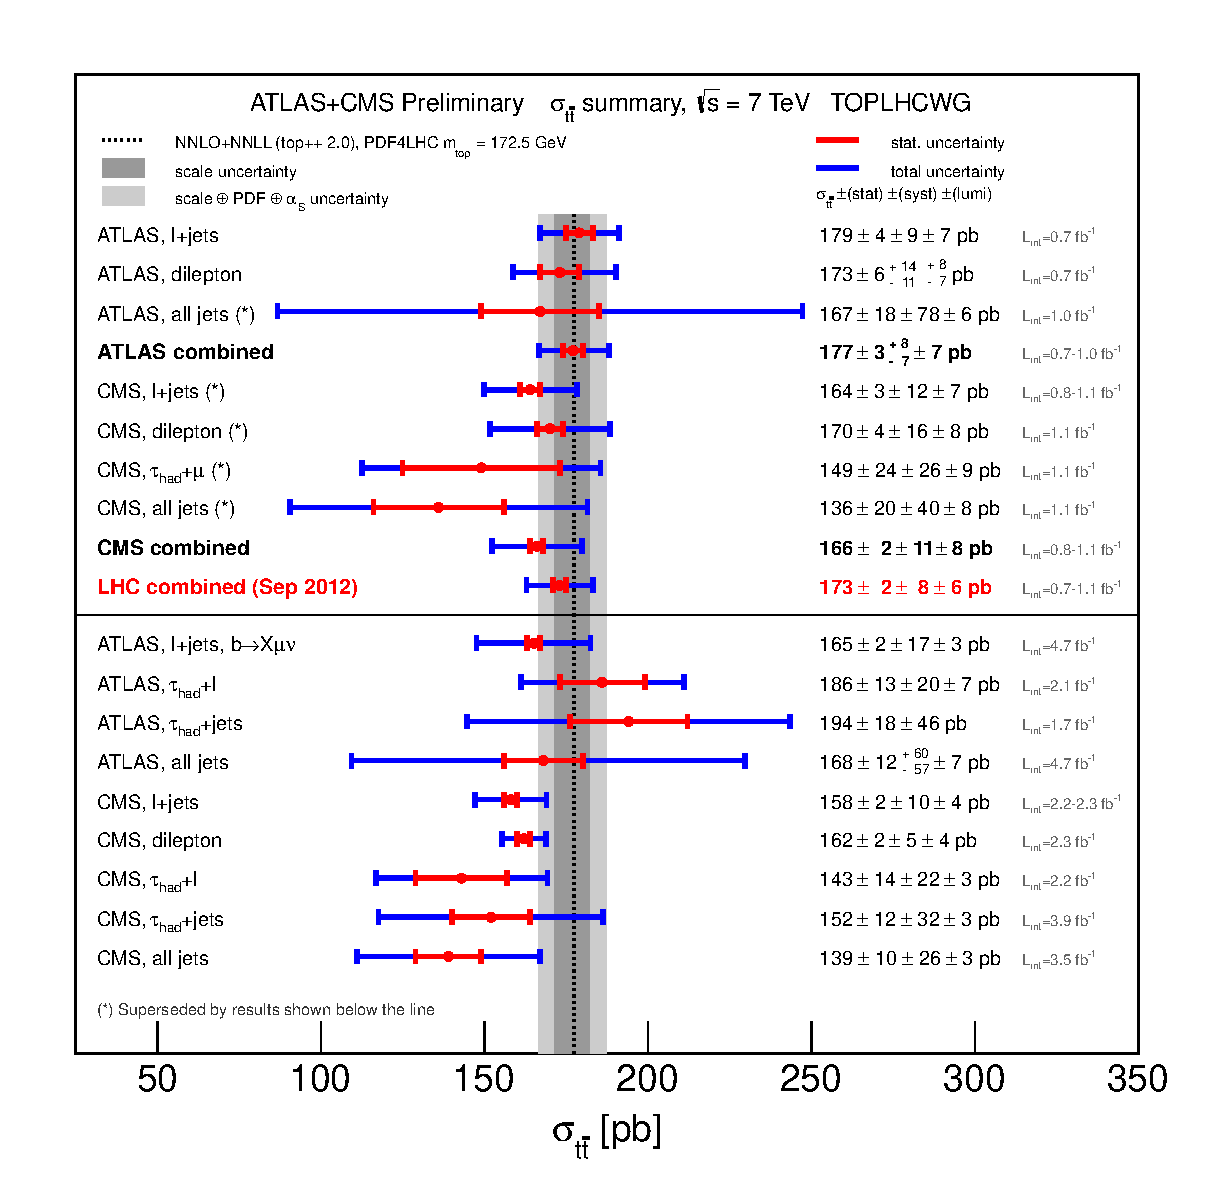
\includegraphics[width=0.95\textwidth]{PartTopQuark/Plots/tt_xsec_7TeV.eps}
  \caption{A summary of all \ttbar\ production cross section measurements performed at the LHC at $\sqrt{s}=7$ TeV. Note the theory prediction shown as a dotted black line with its associated uncertainties as grey bands. The results shown above the black line have been statistically combined, producing the results labelled as \textbf{combined}. Many of these analyses have been superseded and the results are shown below the line. Other analyses performed but not included in the combination are also shown below the line.}
  \label{fig:TopQuarkPairProductionSummaryLHC}
\end{figure}

\begin{figure}[htbp]
  \centering
  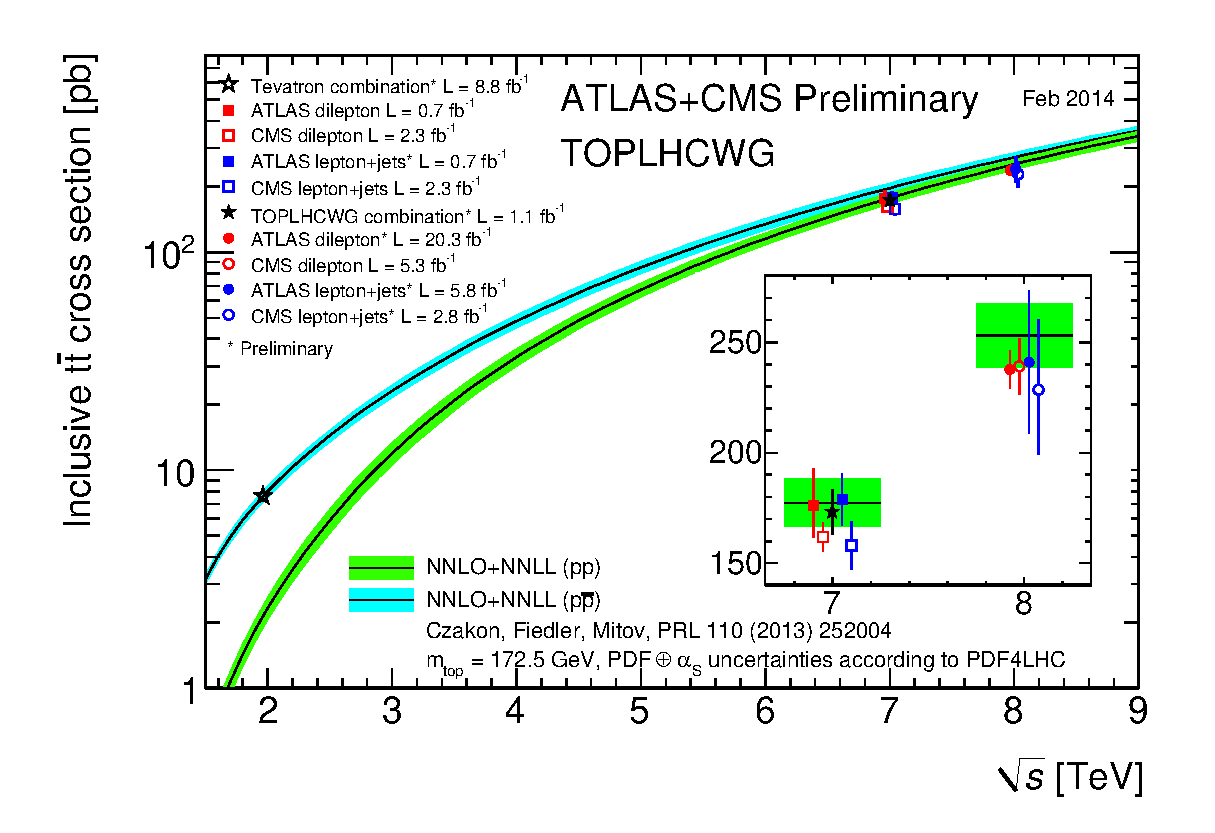
\includegraphics[width=0.95\textwidth]{PartTopQuark/Plots/tt_xsec_vsroots.eps}
  \caption{A summary of the most precise \ttbar\ production cross section measurements performed at the LHC at $\sqrt{s}=$ 7 and 8 TeV and the Tevatron at $\sqrt{s}=1.96$ TeV compared to the theoretical prediction. Note that the Tevatron results should be compared against the prediction for $p\bar{p}$ collisions while the LHC against the $pp$ collision predictions.}
  \label{fig:TopQuarkPairProductionComparison}
\end{figure}

\subsubsection{Mass asymmetry measurement}

As mentioned in Section~\ref{sec:TheoryWeakInteractions}, the charge ($C$) and parity ($P$) symmetries are both violated in weak interactions. The CPT symmetry which includes time reversal ($T$) is the last remaining symmetry which no interaction appears to violate. Any deviations from this symmetry would have major implications on particles physics~\cite{TopQuark:CPTViolation} and could manifest itself as differences between matter and antimatter particles. As the only quark which can be studied directly, measurement of $\Delta m\equiv m_{t}-m_{\bar{t}}$ could hint at any such deviation produced by new physics. Such a measurement was conducted by the ATLAS~\cite{TopQuark:MassAsymmetryATLAS2014} experiment yielding the result:
%
\begin{equation}
  \Delta m_{t}=-0.44\pm0.46\text{ (stat)}\pm0.27\text{ (stat) GeV}
\end{equation}
%
and by the CMS~\cite{TopQuark:MassAsymmetryCMS2012} experiment yielding the result:
%
\begin{equation}
  \Delta m_{t}=0.67\pm0.61\text{ (stat)}\pm0.41\text{ (stat) GeV}
\end{equation}
%
which are both consistent with the SM prediction and imply CPT invariance.

\subsubsection{Charge asymmetry}

Many BSM theories can affect the charge symmetry between top and antitop quarks. Once again any deviations from the SM prediction would point to the existence of new BSM physics. The charge asymmetry as measured by the ATLAS experiment~\cite{TopQuark:ChargeAsymmetryATLAS} is
\begin{equation}
  A_{c}=0.006\pm0.010
\end{equation}
%
and as measured by CMS~\cite{TopQuark:ChargeAsymmetryCMS}
%
\begin{equation}
  A_{c}=-0.010\pm0.017\text{ (stat)}\pm0.008\text{ (syst)}
\end{equation}
%
which once again are consistent with the SM prediction.


